%%%%%%%%%%%%%%%%%%%%%%%%%%%%%%%%%%%%%%%%%
% Short Sectioned Assignment LaTeX Template Version 1.0 (5/5/12)
% This template has been downloaded from: http://www.LaTeXTemplates.com
% Original author:  Frits Wenneker (http://www.howtotex.com)
% License: CC BY-NC-SA 3.0 (http://creativecommons.org/licenses/by-nc-sa/3.0/)
%%%%%%%%%%%%%%%%%%%%%%%%%%%%%%%%%%%%%%%%%

%----------------------------------------------------------------------------------------
%	PACKAGES AND OTHER DOCUMENT CONFIGURATIONS
%----------------------------------------------------------------------------------------

\documentclass[paper=a4, fontsize=11pt]{scrartcl} % A4 paper and 11pt font size

% ---- Entrada y salida de texto -----

\usepackage[T1]{fontenc} % Use 8-bit encoding that has 256 glyphs
\usepackage[utf8]{inputenc}
%\usepackage{fourier} % Use the Adobe Utopia font for the document - comment this line to return to the LaTeX default

% ---- Idioma --------

\usepackage[spanish, es-tabla]{babel} % Selecciona el español para palabras introducidas automáticamente, p.ej. "septiembre" en la fecha y especifica que se use la palabra Tabla en vez de Cuadro

% ---- Otros paquetes ----

\usepackage{url} % ,href} %para incluir URLs e hipervínculos dentro del texto (aunque hay que instalar href)
\usepackage{hyperref}
\hypersetup{
	colorlinks=true,
	linkcolor=black,
	urlcolor=black,
	citecolor=black,
}
\usepackage{amsmath,amsfonts,amsthm} % Math packages
%\usepackage{graphics,graphicx, floatrow} %para incluir imágenes y notas en las imágenes
\usepackage{graphics,graphicx, float} %para incluir imágenes y colocarlas

% Para hacer tablas comlejas
%\usepackage{multirow}
%\usepackage{threeparttable}

%\usepackage{sectsty} % Allows customizing section commands
%\allsectionsfont{\centering \normalfont\scshape} % Make all sections centered, the default font and small caps

\usepackage{fancyhdr} % Custom headers and footers
\pagestyle{fancyplain} % Makes all pages in the document conform to the custom headers and footers
\fancyhead{} % No page header - if you want one, create it in the same way as the footers below
\fancyfoot[L]{} % Empty left footer
\fancyfoot[C]{} % Empty center footer
\fancyfoot[R]{\thepage} % Page numbering for right footer
\renewcommand{\headrulewidth}{0pt} % Remove header underlines
\renewcommand{\footrulewidth}{0pt} % Remove footer underlines
\setlength{\headheight}{13.6pt} % Customize the height of the header

\numberwithin{equation}{section} % Number equations within sections (i.e. 1.1, 1.2, 2.1, 2.2 instead of 1, 2, 3, 4)
\numberwithin{figure}{section} % Number figures within sections (i.e. 1.1, 1.2, 2.1, 2.2 instead of 1, 2, 3, 4)
\numberwithin{table}{section} % Number tables within sections (i.e. 1.1, 1.2, 2.1, 2.2 instead of 1, 2, 3, 4)

\setlength\parindent{0pt} % Removes all indentation from paragraphs - comment this line for an assignment with lots of text

\newcommand{\horrule}[1]{\rule{\linewidth}{#1}} % Create horizontal rule command with 1 argument of height
\usepackage{booktabs}

\usepackage{listings}
\usepackage{color}
\usepackage{xcolor}
\lstdefinestyle{customc}{
	belowcaptionskip=1\baselineskip,
	breaklines=true,
	frame=L,
	xleftmargin=\parindent,
	language=C,
	showstringspaces=false,
	basicstyle=\footnotesize\ttfamily,
	keywordstyle=\bfseries\color{green!40!black},
	commentstyle=\itshape\color{purple!40!black},
	identifierstyle=\color{blue},
	stringstyle=\color{orange},
}

\lstset{escapechar=@,style=customc}
\usepackage{url}

\title{	
	\normalfont \normalsize
	\begin{figure}[htb]
		\centering
		
\includegraphics[width=0.3\textwidth]{./imagenes/1}
	\end{figure}
	\textsc{\textbf{Inteligencia de Negocio} \\ Grado en Ingeniería Informática \\ Universidad de Granada \\
	Curso 2018-2019} \\ [25pt] % Your university, school and/or department name(s)
	\begin{figure}[htb]
		\centering
		
\includegraphics[width=0.15\textwidth]{./imagenes/2}
	\end{figure}
	\horrule{0.5pt} \\[0.4cm] % Thin top horizontal rule
	\huge Memoria Práctica 3. Grupo 1 \\
	\huge Competición en DrivenData.
	\\ % The assignment title
	\horrule{2pt} \\[0.5cm] % Thick bottom horizontal rule
}
\author{Félix Ramírez García  \\
\href{mailto:felixramirezgarcia@correo.ugr.es}{felixramirezgarcia@correo.ugr.es}} % Nombre y apellidos
\date{\normalsize\today} % Incluye la fecha actual

%----------------------------------------------------------------------------------------
% DOCUMENTO
%----------------------------------------------------------------------------------------

\begin{document}
	
	\maketitle % Muestra el Título
	
	\newpage %inserta un salto de página
	
	\begin{figure}[htb]
		\centering
		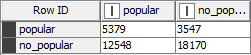
\includegraphics[width=1.0\textwidth]{./imagenes/5}
		\label{fig:1}
	\end{figure}
	
	\newpage %inserta un salto de página
	
	\tableofcontents % para generar el índice de contenidos
	
	\listoffigures % para generar índice de imágenes.
	
	\listoftables % para generar índice de tablas.
	
	\newpage

	%----------------------------------------------------------------------
	%							Introducción
	%----------------------------------------------------------------------	
	
	\section[Introducción]{Introducción.}
	
	Esta practica ha sido llevada a cabo para la asignatura Inteligencia del Negocio de la universidad de Granada, asignatura de cuarto curso del Grado en Ingeniería Informática. En ella veremos el uso de algoritmos de aprendizaje supervisado en clasificación sobre la competición Pump it Up de la plataforma DrivenData . Usaremos un conjunto de datos de Taarifa y del Ministerio de agua de Tanzania para predecir que bombas de agua son funcionales , cuales necesitan reparaciones y cuales no funcionan. Se trata de una competición para la comprensión de los puntos de agua que fallaran , pudiendo así mejorar las operaciones de mantenimiento. \\
	
	El conjunto de datos de entrenamiento tiene 59400 instancias y para predecir una de las tres clases se dispone de 39 variables. Las variables son las siguientes:\\
	
	amount\_tsh - cantidad de agua disponible para el punto de agua \\
	date\_recorded - La fecha en que se introdujo la fila \\				
	funder - Quién financió el pozo \\
	gps\_height - Altitud del pozo \\
	installer - Organización que instaló el pozo \\
	longitude - Coordenada GPS \\
	latitude - Coordenada GPS\\
	wpt\_name - Nombre del punto de agua si hay uno \\
	num\_private - Numero privado\\
	basin - Cuenca geográfica\\
	subvillage - Ubicación geográfica\\
	region - Ubicación geográfica \\
	region\_code - Ubicación geográfica (coded)\\
	district\_code - Ubicación geográfica (coded)\\
	lga - Ubicación geográfica\\
	ward - Ubicación geográfica\\
	population - Población alrededor del pozo\\
	public\_meeting - Verdadero/Falso\\
	recorded\_by - Grupo que introduce esta fila de datos\\
	scheme\_management - Quién opera el punto de agua\\
	scheme\_name - Quién opera el punto de agua\\
	permit - Si el punto de agua está permitido\\
	construction\_year - Año de construcción del punto de agua \\
	extraction\_type - El tipo de extracción que utiliza el punto de agua\\
	extraction\_type\_group - El tipo de extracción que utiliza el punto de agua\\
	extraction\_type\_class - El tipo de extracción que utiliza el punto de agua\\
	management - Cómo se gestiona el punto de agua\\
	management\_group - Cómo se gestiona el punto de agua\\
	payment - Lo que cuesta el agua\\
	payment\_type - Lo que cuesta el agua \\
	water\_quality - La calidad del agua\\
	quality\_group - La calidad del agua\\
	quantity - La cantidad de agua\\
	quantity\_group - La cantidad de agua\\
	source - La fuente del agua\\
	source\_type - La fuente del agua\\
	source\_class - La fuente del agua\\
	waterpoint\_type - El tipo de punto de agua\\
	waterpoint\_type\_group - El tipo de punto de agua\\
	
	La práctica consiste en competir entre los distintos alumnos de la asignatura , de forma que debemos con cada subida a DrivenData describir el objetivo de las modificaciones realizadas sobre el Script y explicar el preprocesamiento de los datos y la elección de los parámetros de los algoritmos. En la competición se emplea el porcentaje de acierto como Score para valorar la calidad de la solución aportada.\\
	
	Por último cabe decir que anexo a esta documentación se proporcionan los Scripts realizados para cada subida y el archivo formato csv con los resultados generados. \\
	
	%----------------------------------------------------------------------
	%					Progreso de la competición
	%----------------------------------------------------------------------	
	
	\section[Progreso de la competición]{Progreso de la competición.}
	
	En este apartado se expone el progreso llevado a cabo para la competición en DrivenData, introduciendo partes del código y tablas correspondientes a cada subida durante la competición. \\
	
	%----------------------------------------------------------------------
	%						Subida numero 1
	%----------------------------------------------------------------------	
	
	\subsection[Subida numero 1]{Subida numero 1.}
	
	En esta primera subida se ha hecho uso del Script proporcionado por el profesor de Practicas de la asignatura, y en mi caso las mejoras realizadas se basan en modificaciones sobre este primer fichero de prueba. Estas mejoras son modificaciones del pre-procesamiento, modificaciones de los parámetros de los algoritmos, o directamente sustituir un algoritmo por otro. \\
	
	A continuación mostramos el Script completo para esta primera subida, pero  en las siguientes secciones solamente se mostraran aquellas modificaciones 
	realizadas sobre este programa. 
	
	\lstset{language=python}
	\begin{lstlisting}[frame=single]
'''
###########################################################
IMPORTS
###########################################################
'''
import pandas as pd
import numpy as np
import time
from sklearn.model_selection import StratifiedKFold
from sklearn.metrics import accuracy_score
from sklearn import preprocessing
from sklearn.ensemble import RandomForestRegressor
import xgboost as xgb
import lightgbm as lgb
from sklearn.preprocessing import LabelEncoder

from sklearn.metrics import make_scorer
from sklearn.model_selection import GridSearchCV
from sklearn.model_selection import RandomizedSearchCV

'''
############################################################
FUNCIONES
############################################################
'''
def validacion_cruzada(modelo, X, y, cv):
	y_test_all = []
	
	for train, test in cv.split(X, y):
	t = time.time()
	modelo = modelo.fit(X[train],y[train])
	tiempo = time.time() - t
	y_pred = modelo.predict(X[test])
	print("Score: {:.4f}, tiempo: {:6.2f} segundos".format(accuracy_score(y[test],y_pred) , tiempo))
	y_test_all = np.concatenate([y_test_all,y[test]])
	
	print("")
	
	return modelo, y_test_all

'''
############################################################
LECTURA DE DATOS
############################################################
'''
#los ficheros .csv se han preparado previamente para sustituir ,, y "Not known" por NaN (valores perdidos)
carpeta_datos="C:/Users/felix/Desktop/Google-Drive/IN/Practica3/dataset/"
# Datos training
data_x_tra = pd.read_csv(carpeta_datos+'water_pump_tra.csv',na_values="unknown")
# La clasificacion
data_y = pd.read_csv(carpeta_datos+'water_pump_tra_target.csv')
# Datos test
data_x_tst = pd.read_csv(carpeta_datos+'water_pump_tst.csv',na_values="unknown")

'''
############################################################
ELIMINACION DE COLUMNAS
############################################################
'''
################# eliminar id ###################################
data_x_tra.drop(labels=['id'], axis=1,inplace = True)
data_x_tra.drop(labels=['date_recorded'], axis=1,inplace = True)
data_x_tst.drop(labels=['id'], axis=1,inplace = True)
data_x_tst.drop(labels=['date_recorded'], axis=1,inplace = True)
data_y.drop(labels=['id'], axis=1,inplace = True)

'''
############################################################
CATEGORICAS A NUMERICAS
############################################################
'''
######################### TRAINING ##############################
mask = data_x_tra.isnull()  #mascara para luego recuperar los NaN
data_x_tmp = data_x_tra.fillna(9999) # Combierte los NaN en 9999
data_x_tmp = data_x_tmp.astype(str).apply(LabelEncoder().fit_transform) #se convierten categoricas en numericas
data_x_tra_nan = data_x_tmp.where(~mask, data_x_tra)  #se recuperan los NaN

############################# TEST ##############################
mask = data_x_tst.isnull() #mascara para luego recuperar los NaN
data_x_tmp = data_x_tst.fillna(9999) #LabelEncoder no funciona con NaN, se asigna un valor no usado
data_x_tmp = data_x_tmp.astype(str).apply(LabelEncoder().fit_transform) #se convierten categoricas en numericas
data_x_tst_nan = data_x_tmp.where(~mask, data_x_tst) #se recuperan los NaN

X_tra = data_x_tra_nan.values
X_tst = data_x_tst_nan.values
y = np.ravel(data_y.values)
'''
############################################################
ALGORITMOS
############################################################
'''
#Validacion cruzada con particionado estratificado y control de la aleatoriedad fijando la semilla
skf = StratifiedKFold(n_splits=5, shuffle=True, random_state=123456)
df_submission = pd.read_csv(carpeta_datos+'water_pump_submissionformat.csv')

#------------------------------ XGB ---------------------------------------
print("------ XGB ------")
gradient = xgb.XGBClassifier(n_estimators = 200)
gradient,y_test_gradient = validacion_cruzada(gradient,X_tra,y,skf)
gradient = gradient.fit(X_tra,y)
y_pred_tra_gradient = gradient.predict(X_tra)
print("Score XGB: {:.4f}".format(accuracy_score(y,y_pred_tra_gradient)))
y_pred_tst_gradient = gradient.predict(X_tst)
df_submission['status_group'] = y_pred_tst_gradient
df_submission.to_csv("submission_gradient.csv", index=False)

#----------------------------- LightGBM -------------------------------------
print("------ LightGBM ------")
light = lgb.LGBMClassifier(objective='binary',n_estimators=200,num_threads=2)
ligth, y_test_lgbm = validacion_cruzada(light,X_tra,y,skf)
ligth = ligth.fit(X_tra,y)
y_pred_tra_ligth = ligth.predict(X_tra)
print("Score LightGBM: {:.4f}".format(accuracy_score(y,y_pred_tra_ligth)))
y_pred_tst_ligth = ligth.predict(X_tst)
df_submission['status_group'] = y_pred_tst_ligth
df_submission.to_csv("submission_ligth.csv", index=False)
	\end{lstlisting}
	
	
	%----------------------------------------------------------------------
	%			Preprocesamiento y algoritmos usados Subida 1
	%----------------------------------------------------------------------	
	
	\subsubsection[Preprocesamiento y algoritmos usados Subida 1]{Preprocesamiento y algoritmos usados Subida 1}
	
	Al comienzo de este Script creamos tres variables , una para almacenar el conjunto de datos para entrenamiento, otra para el conjunto de datos de test , y otra para almacenar el target del entrenamiento. Pasamos a eliminar la columna del identificador 'id' de estas tres variables, y también eliminamos la columna 'date\_recorded' del training y del test. Después pasamos a convertir las variables categóricas a numéricas (ordinales) mientras que conservamos los valores perdidos (NaN). Por ultimo ejecutamos los algoritmos XGB y LightGBM usando una validación cruzada con particionamiento estratificado y control de la aleatoriedad fijando la semilla. El parámetro usado para el algoritmos XGB es:\\
	
	n\_estimators = 200 \\
	
	Y los parámetros usados para el algoritmo LightGBM son\\
	
	objective = 'binary'\\
	n\_estimators = 200\\
	num\_threads = 2\\
	
	A continuación se muestran los resultados obtenidos en cada validación para los dos algoritmos:
	
	------ XGB ------ 			   		   \\
	Score: 0.7618, tiempo:  84.87 segundos \\
	Score: 0.7604, tiempo:  97.93 segundos \\
	Score: 0.7597, tiempo:  99.20 segundos \\
	Score: 0.7583, tiempo: 101.06 segundos \\
	Score: 0.7579, tiempo: 101.60 segundos \\
	
	La media de las 5 validaciones para el algoritmo XGB es : 0.7596 \\
	
	---- LightGBM ----					    \\		
	Score: 0.7992, tiempo:   9.93 segundos  \\
	Score: 0.7941, tiempo:   9.24 segundos  \\
	Score: 0.7927, tiempo:   9.37 segundos  \\
	Score: 0.7961, tiempo:   9.11 segundos  \\
	Score: 0.7925, tiempo:  10.12 segundos  \\
	
	La media de las 5 validaciones para el algoritmo LightGBM es : 0.7949 \\
	
	Ya que el resultado obtenido por el algoritmo LightGBM es mejor lo usamos para la subida a la plataforma DrivenData.
	
	%----------------------------------------------------------------------
	%						Subida numero 2
	%----------------------------------------------------------------------	
	
	\subsection[Subida numero 2]{Subida numero 2.}
	
	El fragmento de código Python modificado respecto a la anterior subida es el siguiente:
	
	\lstset{language=python}
	\begin{lstlisting}[frame=single]
params_lgbm = {
	'feature_fraction':[i/10.0 for i in range(2,3)],
	'learning_rate':[i/100.0 for i in range(1,2)],
	'num_leaves':[i for i in range(195,200)],
	'n_estimators':[i*10 for i in range(195,250)]
}
grid_lgbm = GridSearchCV(light, params_lgbm, cv=3, n_jobs=1, verbose=1, scoring=acc_scorer)
grid_lgbm.fit(X_tra,y)
print(grid_lgbm.best_params_)
gs_lgbm, y_test_gs = validacion_cruzada(grid_lgbm.best_estimator_,X_tra,y,skf)
gs_lgbm = gs_lgbm.fit(X_tra,y)
y_pred_tra_ligth = gs_lgbm.predict(X_tra)
	\end{lstlisting}
	
	%----------------------------------------------------------------------
	%			Preprocesamiento y algoritmos usados Subida 2
	%----------------------------------------------------------------------	
	
	\subsubsection[Preprocesamiento y algoritmos usados Subida 2]{Preprocesamiento y algoritmos usados Subida 2}
	
	En esta segunda subida se ha descartado el algoritmo XGB y se han realizado modificaciones 
	sobre el algoritmo LightGBM , que parece mas rápido y preciso. Estas modificaciones han 
	sido para optimizar la elección de parámetros para el algoritmo, y para ello se ha usado 
	una Grid Search. Después de la ejecucion se han obtenido como mejores (dentro de los 
	rangos indicados) valores de parámetros para el algoritmo: \\
	
	feature\_fraction : 0.3 \\
	learning\_rate : 0.01 \\
	num\_leaves : 200 \\
	n\_estimators : 2500 \\
	
	El preprocesamiento se mantiene respecto a la subida anterior, es decir, simplemente eliminamos las columnas id y date\_recorded  y pasamos las variables 
	categóricas a numéricas. A continuación se muestran los resultados obtenidos para cada validación en el algoritmo LightGBM: \\
	
	------ LightGBM ------\\
	Score: 0.7947, tiempo:  12.52 segundos \\
	Score: 0.7919, tiempo:  12.74 segundos \\
	Score: 0.7923, tiempo:  12.56 segundos \\
	Score: 0.7919, tiempo:  12.56 segundos \\
	Score: 0.7910, tiempo:  12.69 segundos \\  
	
	La media de las 5 validaciones para el algoritmo LightGBM es 0.7923:  \\

	%----------------------------------------------------------------------
	%						Subida numero 3
	%----------------------------------------------------------------------	
	
	\subsection[Subida numero 3]{Subida numero 3.}
	
	El fragmento de código Python modificado respecto a la anterior subida es el siguiente:
	
	\lstset{language=python}
	\begin{lstlisting}[frame=single]
gradient = xgb.XGBClassifier(n_estimators = 200)

print("------ Grid Search XGB -------")
params_xgb = {
	'min_child_weight':[4,5],
	'gamma':[i/10.0 for i in range(3,6)],
	'subsample':[i/10.0 for i in range(6,11)],
	'colsample_bytree':[i/10.0 for i in range(6,11)],
	'max_depth': [2,3,4],
	'n_estimators':[50,100,200]
}
grid_xgb = GridSearchCV(gradient, params_xgb, cv=3, n_jobs=1, verbose=1, scoring=acc_scorer)
grid_xgb.fit(X_tra,y)

print("------Mejores parametros XGB-----:")
print(grid_xgb.best_params_)
gs_xgb, y_test_gs = validacion_cruzada(grid_xgb.best_estimator_,X_tra,y,skf)
gs_xgb = gs_xgb.fit(X_tra,y)
y_pred_tra_xgb = gs_xgb.predict(X_tra)
	\end{lstlisting}
	
	%----------------------------------------------------------------------
	%			Preprocesamiento y algoritmos usados Subida 3
	%----------------------------------------------------------------------	
	
	\subsubsection[Preprocesamiento y algoritmos usados Subida 3]{Preprocesamiento y algoritmos usados Subida 3}
	
	En esta segunda subida se le vuelve a dar una oportunidad al algoritmo XGB .Se le han realizado
	modificaciones respecto al usado en la subida 1 para optimizar la elección de parámetros para el algoritmo, 
	y para ello se ha usado una Grid Search. Después de la ejecucion se han obtenido como mejores (dentro de los 
	rangos indicados) valores de parámetros para el algoritmo: \\
	
	min\_child\_weight=4\\
	gamma=0.3\\
	subsample=0.6\\
	colsample\_bytree=0.6\\
	max\_depth=4\\
	n\_estimators = 200\\
	
	El preprocesamiento se mantiene respecto a la subida anterior, es decir, simplemente eliminamos las columnas id y date\_recorded  y pasamos las variables 
	categóricas a numéricas. A continuación se muestran los resultados obtenidos para cada validación en el algoritmo LightGBM: \\
	
	------ XGB ------\\
	Score: 0.7765, tiempo:  52.95 segundos \\ 
	Score: 0.7785, tiempo:  53.20 segundos \\
	Score: 0.7753, tiempo:  53.00 segundos \\
	Score: 0.7746, tiempo:  52.84 segundos \\
	Score: 0.7734, tiempo:  53.27 segundos \\
	
	La media de las 5 validaciones para el algoritmo XGB es 0.7756:  \\

	%----------------------------------------------------------------------
	%						Subida numero 4
	%----------------------------------------------------------------------	
	
	\subsection[Subida numero 4]{Subida numero 4.}
	
	El fragmento de código Python modificado respecto a la anterior subida es el siguiente:
	
	\lstset{language=python}
	\begin{lstlisting}[frame=single]
################# Training ###################
data_x_tra.drop(labels=['id'], axis=1,inplace = True)
data_x_tra.drop(labels=['date_recorded'], axis=1,inplace = True)
data_x_tra.drop(labels=['longitude'], axis=1,inplace = True)
data_x_tra.drop(labels=['latitude'], axis=1,inplace = True)
data_x_tra.drop(labels=['wpt_name'], axis=1,inplace = True)
data_x_tra.drop(labels=['num_private'], axis=1,inplace = True)
################# Test  #######################
data_x_tst.drop(labels=['id'], axis=1,inplace = True)
data_x_tst.drop(labels=['date_recorded'], axis=1,inplace = True)
data_x_tst.drop(labels=['longitude'], axis=1,inplace = True)
data_x_tst.drop(labels=['latitude'], axis=1,inplace = True)
data_x_tst.drop(labels=['wpt_name'], axis=1,inplace = True)
data_x_tst.drop(labels=['num_private'], axis=1,inplace = True)
################# Target  ######################
data_y.drop(labels=['id'], axis=1,inplace = True)


print("------ LightGBM ------")
light = lgb.LGBMClassifier(feature_fraction=0.3,learning_rate=0.01,n_estimators=2500,num_leaves=200)
ligth, y_test_lgbm = validacion_cruzada(light,X_tra,y,skf)
ligth = ligth.fit(X_tra,y)
y_pred_tra_ligth = ligth.predict(X_tra)
print("Score LightGBM: {:.4f}".format(accuracy_score(y,y_pred_tra_ligth)))
y_pred_tst_ligth = ligth.predict(X_tst)
df_submission['status_group'] = y_pred_tst_ligth
df_submission.to_csv("submission_ligth.csv", index=False)
	\end{lstlisting}
	
	%----------------------------------------------------------------------
	%			Preprocesamiento y algoritmos usados Subida 4
	%----------------------------------------------------------------------	
	
	\subsubsection[Preprocesamiento y algoritmos usados Subida 4]{Preprocesamiento y algoritmos usados Subida 4}
	
	En esta cuarta subida se ha descartado el algoritmo XGB por sus malos resultados en comparación a
	LightGBM y se han realizado modificaciones 
	sobre el algoritmo LightGBM , ajustando los parámetros a los obtenidos al realizar la Grid Search
	de la subida 2. Los parámetros usados para el algoritmo LightGBM son: \\
	
	feature\_fraction : 0.3 \\
	learning\_rate : 0.01 \\
	num\_leaves : 200 \\
	n\_estimators : 2400 \\
	
	Ahora en el preprocesamiento eliminamos las columnas anteriores de id y date\_recorded, y ademas eliminamos
	las columnas longitude, latitude , wpt\_name y num\_private. A continuación se muestran los resultados 
	obtenidos para cada validación en el algoritmo LightGBM: \\

	------ LightGBM ------\\
	Score: 0.8130, tiempo:  73.63 segundos\\
	Score: 0.8131, tiempo:  75.45 segundos\\
	Score: 0.8120, tiempo:  74.56 segundos\\
	Score: 0.8140, tiempo:  81.78 segundos\\
	Score: 0.8104, tiempo:  77.39 segundos\\
	
	La media de las 5 validaciones para el algoritmo LightGBM es 0.8125:  \\

	%----------------------------------------------------------------------
	%						Subida numero 5
	%----------------------------------------------------------------------	
	
	\subsection[Subida numero 5]{Subida numero 5.}
	
	El fragmento de código Python modificado respecto a la anterior subida es el siguiente:
	
	\lstset{language=python}
	\begin{lstlisting}[frame=single]
data_x_tra['amount_tsh'] = data_x_tra['amount_tsh'].apply(pd.to_numeric, errors='coerce')
data_x_tra.replace({'amount_tsh' : 0}, 1000, inplace=True)
data_x_tst['amount_tsh'] = data_x_tst['amount_tsh'].apply(pd.to_numeric, errors='coerce')
data_x_tst.replace({'amount_tsh' : 0}, 1000, inplace=True)
	\end{lstlisting}
	
	%----------------------------------------------------------------------
	%			Preprocesamiento y algoritmos usados Subida 5
	%----------------------------------------------------------------------	
	
	\subsubsection[Preprocesamiento y algoritmos usados Subida 5]{Preprocesamiento y algoritmos usados Subida 5}
	
	En esta quinta subida se ha usado el algoritmo LightGBM y se han realizado modificaciones 
	en el preprocesamiento , sustituyendo los valores de cero en la columna amount\_tsh
	por 1000. Los parámetros usados para el algoritmo LightGBM son los mismos que la subida anterior: \\
	
	feature\_fraction : 0.3 \\
	learning\_rate : 0.01 \\
	num\_leaves : 200 \\
	n\_estimators : 2400 \\
	
	En el preprocesamiento eliminamos al igual que en la subida anterior las columnas de id , date\_recorded,
	longitude, latitude , wpt\_name y num\_private. A continuación se muestran los resultados 
	obtenidos para cada validación en el algoritmo LightGBM: \\

	------ LightGBM ------\\
	Score: 0.8119, tiempo:  74.78 segundos \\
	Score: 0.8129, tiempo:  75.07 segundos \\
	Score: 0.8102, tiempo:  74.75 segundos \\
	Score: 0.8140, tiempo:  73.86 segundos \\
	Score: 0.8096, tiempo:  73.99 segundos \\
	
	La media de las 5 validaciones para el algoritmo LightGBM es 0.8117 , peor que la anterior subida, por lo 
	que descartamos este cambio.  \\

	%----------------------------------------------------------------------
	%						Subida numero 6
	%----------------------------------------------------------------------	
	
	\subsection[Subida numero 6]{Subida numero 6.}
	
	El fragmento de código Python modificado respecto a la anterior subida es el siguiente:
	
	\lstset{language=python}
	\begin{lstlisting}[frame=single]
data_x_tra['amount_tsh'] = data_x_tra['amount_tsh'].apply(pd.to_numeric, errors='coerce')
data_x_tra.replace({'amount_tsh' : 0}, 2000, inplace=True)
data_x_tst['amount_tsh'] = data_x_tst['amount_tsh'].apply(pd.to_numeric, errors='coerce')
data_x_tst.replace({'amount_tsh' : 0}, 2000, inplace=True)


tipos = data_x_tra.columns.to_series().groupby(data_x_tra.dtypes).groups
ctext = tipos[np.dtype('object')]

columnas = data_x_tra.columns  
cnum = list(set(columnas) - set(ctext))

for c in cnum:
	mean = data_x_tra[c].mean()
	data_x_tra[c] = data_x_tra[c].fillna(mean)
	data_x_tst[c] = data_x_tst[c].fillna(mean)
	
for c in ctext:
	mode = data_x_tra[c].mode()[0]
	data_x_tra[c] = data_x_tra[c].fillna(mode)
	data_x_tst[c] = data_x_tst[c].fillna(mode)
	\end{lstlisting}
	
	%----------------------------------------------------------------------
	%			Preprocesamiento y algoritmos usados Subida 6
	%----------------------------------------------------------------------	
	
	\subsubsection[Preprocesamiento y algoritmos usados Subida 6]{Preprocesamiento y algoritmos usados Subida 6}
	
	En esta sexta subida se ha usado el algoritmo LightGBM y se han realizado modificaciones 
	en el preprocesamiento , sustituyendo los valores de cero en la columna amount\_tsh
	por 2000 , rellenando los valores perdidos de las variables categóricas con la moda y de las 
	variables numericas con la media. Los parámetros usados para el algoritmo LightGBM son los mismos que la subida anterior: \\
	
	feature\_fraction : 0.3 \\
	learning\_rate : 0.01 \\
	num\_leaves : 200 \\
	n\_estimators : 2400 \\
	
	En el preprocesamiento eliminamos al igual que en la subida anterior las columnas de id , date\_recorded,
	longitude, latitude , wpt\_name y num\_private. A continuación se muestran los resultados 
	obtenidos para cada validación en el algoritmo LightGBM: \\

	------ LightGBM ------\\
	Score: 0.8103, tiempo:  66.72 segundos\\
	Score: 0.8141, tiempo:  66.40 segundos\\
	Score: 0.8094, tiempo:  65.41 segundos\\
	Score: 0.8123, tiempo:  67.16 segundos\\
	Score: 0.8095, tiempo:  65.74 segundos\\
	
	La media de las 5 validaciones para el algoritmo LightGBM es 0.8111 , peor que la anterior subida, por lo 
	que descartamos este cambio.  \\

	%----------------------------------------------------------------------
	%						Subida numero 7
	%----------------------------------------------------------------------	
	
	\subsection[Subida numero 7]{Subida numero 7.}
	
	El fragmento de código Python modificado respecto a la anterior subida es el siguiente:
	
	\lstset{language=python}
	\begin{lstlisting}[frame=single]
################# Training ###################
data_x_tra.drop(labels=['id'], axis=1,inplace = True)
data_x_tra.drop(labels=['date_recorded'], axis=1,inplace = True)
data_x_tra.drop(labels=['longitude'], axis=1,inplace = True)
data_x_tra.drop(labels=['latitude'], axis=1,inplace = True)
data_x_tra.drop(labels=['wpt_name'], axis=1,inplace = True)
data_x_tra.drop(labels=['num_private'], axis=1,inplace = True)
data_x_tra.drop(labels=['subvillage'], axis=1,inplace = True)
data_x_tra.drop(labels=['funder'], axis=1,inplace = True)
################ Test  #######################
data_x_tst.drop(labels=['id'], axis=1,inplace = True)
data_x_tst.drop(labels=['date_recorded'], axis=1,inplace = True)
data_x_tst.drop(labels=['longitude'], axis=1,inplace = True)
data_x_tst.drop(labels=['latitude'], axis=1,inplace = True)
data_x_tst.drop(labels=['wpt_name'], axis=1,inplace = True)
data_x_tst.drop(labels=['num_private'], axis=1,inplace = True)
data_x_tst.drop(labels=['subvillage'], axis=1,inplace = True)
data_x_tst.drop(labels=['funder'], axis=1,inplace = True)
################ Target  ######################
data_y.drop(labels=['id'], axis=1,inplace = True)
	\end{lstlisting}
	
	%----------------------------------------------------------------------
	%			Preprocesamiento y algoritmos usados Subida 7
	%----------------------------------------------------------------------	
	
	\subsubsection[Preprocesamiento y algoritmos usados Subida 7]{Preprocesamiento y algoritmos usados Subida 7}
	
	En esta séptima subida se ha usado el algoritmo LightGBM con los mismos
	parámetros usados que la subida anterior: \\
	
	feature\_fraction : 0.3 \\
	learning\_rate : 0.01 \\
	num\_leaves : 200 \\
	n\_estimators : 2400 \\
	
	En el preprocesamiento eliminamos al igual que en la subida anterior las columnas de id , date\_recorded,
	longitude, latitude , wpt\_name y num\_private , pero ahora también eliminamos subvillage
	y funder . A continuación se muestran los resultados 
	obtenidos para cada validación en el algoritmo LightGBM: \\

	------ LightGBM ------\\
	Score: 0.8108, tiempo:  70.20 segundos\\
	Score: 0.8121, tiempo:  68.88 segundos\\
	Score: 0.8073, tiempo:  72.68 segundos\\
	Score: 0.8138, tiempo:  74.73 segundos\\
	Score: 0.8096, tiempo:  76.51 segundos\\
	
	La media de las 5 validaciones para el algoritmo LightGBM es 0.8107 \\

	%----------------------------------------------------------------------
	%						Subida numero 8
	%----------------------------------------------------------------------	
	
	\subsection[Subida numero 8]{Subida numero 8.}
	
	El fragmento de código Python modificado respecto a la anterior subida es el siguiente:
	
	\lstset{language=python}
	\begin{lstlisting}[frame=single]
data_x_tra.drop(labels=['scheme_name'], axis=1,inplace = True)
data_x_tra.drop(labels=['installer'], axis=1,inplace = True)
data_x_tra.drop(labels=['ward'], axis=1,inplace = True)

data_x_tst.drop(labels=['scheme_name'], axis=1,inplace = True)
data_x_tst.drop(labels=['installer'], axis=1,inplace = True)
data_x_tst.drop(labels=['ward'], axis=1,inplace = True)
	\end{lstlisting}
	
	%----------------------------------------------------------------------
	%			Preprocesamiento y algoritmos usados Subida 8
	%----------------------------------------------------------------------	
	
	\subsubsection[Preprocesamiento y algoritmos usados Subida 8]{Preprocesamiento y algoritmos usados Subida 8}
	
	En esta octava subida se ha usado el algoritmo LightGBM con los mismos
	parámetros usados que la subida anterior: \\
	
	feature\_fraction : 0.3 \\
	learning\_rate : 0.01 \\
	num\_leaves : 200 \\
	n\_estimators : 2400 \\
	
	En el preprocesamiento eliminamos al igual que en la subida anterior las columnas de id , date\_recorded,
	longitude, latitude , wpt\_name , num\_private, subvillage y funder . Y a esas le sumamos en esta subida las 
	columnas scheme\_name, installer y ward . A continuación se muestran los resultados 
	obtenidos para cada validación en el algoritmo LightGBM: \\

	------ LightGBM ------\\
	Score: 0.7996, tiempo:  63.07 segundos\\
	Score: 0.8007, tiempo:  64.26 segundos\\
	Score: 0.7949, tiempo:  65.53 segundos\\
	Score: 0.7999, tiempo:  63.40 segundos\\
	Score: 0.8013, tiempo:  64.32 segundos\\
	
	La media de las 5 validaciones para el algoritmo LightGBM es 0.7992 \\

	%----------------------------------------------------------------------
	%						Subida numero 9
	%----------------------------------------------------------------------	
	
	\subsection[Subida numero 9]{Subida numero 9.}
	
	El fragmento de código Python modificado respecto a la anterior subida es el siguiente:
	
	\lstset{language=python}
	\begin{lstlisting}[frame=single]
data_x_tst.drop(labels=['scheme_management'], axis=1,inplace = True)
data_x_tst.drop(labels=['lga'], axis=1,inplace = True)

data_x_tra.drop(labels=['scheme_management'], axis=1,inplace = True)
data_x_tra.drop(labels=['lga'], axis=1,inplace = True)
	\end{lstlisting}
	
	%----------------------------------------------------------------------
	%			Preprocesamiento y algoritmos usados Subida 9
	%----------------------------------------------------------------------	
	
	\subsubsection[Preprocesamiento y algoritmos usados Subida 9]{Preprocesamiento y algoritmos usados Subida 9}
	
	En esta novena subida se ha usado el algoritmo LightGBM con los mismos
	parámetros usados que la subida anterior: \\
	
	feature\_fraction : 0.3 \\
	learning\_rate : 0.01 \\
	num\_leaves : 200 \\
	n\_estimators : 2400 \\
	
	En el preprocesamiento eliminamos al igual que en la subida anterior las columnas de id , date\_recorded,
	longitude, latitude , wpt\_name , num\_private, subvillage y funder ,scheme\_name, installer y ward .Y a esas le sumamos en esta subida las 
	columnas de scheme\_management y lga . A continuación se muestran los resultados 
	obtenidos para cada validación en el algoritmo LightGBM: \\

	------ LightGBM ------\\
	Score: 0.8002, tiempo:  59.48 segundos\\
	Score: 0.7982, tiempo:  61.21 segundos\\
	Score: 0.7961, tiempo:  61.13 segundos\\
	Score: 0.7984, tiempo:  60.89 segundos\\
	Score: 0.7970, tiempo:  61.48 segundos\\
	
	La media de las 5 validaciones para el algoritmo LightGBM es 0.7979 \\

	%----------------------------------------------------------------------
	%						Subida numero 10
	%----------------------------------------------------------------------	
	
	\subsection[Subida numero 10]{Subida numero 10.}
	
	El fragmento de código Python modificado respecto a la anterior subida es la eliminación de las 
	siguientes lineas:
	
	\lstset{language=python}
	\begin{lstlisting}[frame=single]
data_x_tst.drop(labels=['lga'], axis=1,inplace = True)
data_x_tra.drop(labels=['lga'], axis=1,inplace = True)
	\end{lstlisting}
	
	%----------------------------------------------------------------------
	%			Preprocesamiento y algoritmos usados Subida 10
	%----------------------------------------------------------------------	
	
	\subsubsection[Preprocesamiento y algoritmos usados Subida 10]{Preprocesamiento y algoritmos usados Subida 10}
	
	En esta décima subida se ha usado el algoritmo LightGBM con los mismos
	parámetros usados que la subida anterior: \\
	
	feature\_fraction : 0.3 \\
	learning\_rate : 0.01 \\
	num\_leaves : 200 \\
	n\_estimators : 2400 \\
	
	En el preprocesamiento eliminamos al igual que en la subida anterior las columnas de id , date\_recorded,
	longitude, latitude , wpt\_name , num\_private, subvillage , funder ,scheme\_name, installer , ward y
	scheme\_management , y se ha vuelto a contar en el dataset con la columna lga eliminada en la anterior
	subida. A continuación se muestran los resultados 
	obtenidos para cada validación en el algoritmo LightGBM: \\

	------ LightGBM ------\\
	Score: 0.7989, tiempo:  64.56 segundos\\
	Score: 0.7995, tiempo:  65.88 segundos\\
	Score: 0.7965, tiempo:  64.83 segundos\\
	Score: 0.7997, tiempo:  65.88 segundos\\
	Score: 0.7995, tiempo:  63.01 segundos\\
	
	La media de las 5 validaciones para el algoritmo LightGBM es 0.7928 \\

	En las ultimas cuatro subidas se ha ido perdiendo Score en el entrenamiento pero al subir los 
	resultados obtenidos en DrivenData el Score ha ido aumentando.

	%----------------------------------------------------------------------
	%					Tabla final de resultados
	%----------------------------------------------------------------------	
	
	\begin{figure}[htb]
		\centering
		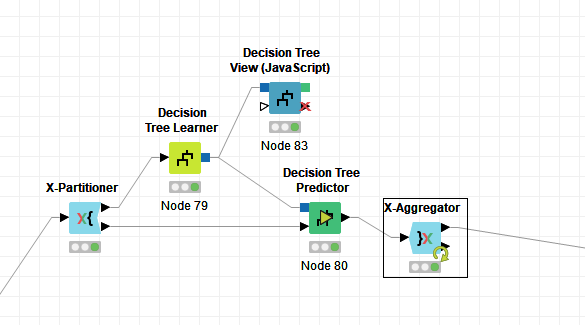
\includegraphics[width=1.0\textwidth]{./imagenes/6}
		\caption{Tabla final de resultados.} \label{fig:1}
	\end{figure}
	
	
	\begin{thebibliography}{99}
		%---------------------------------------
		\bibitem{cite1} 
		\textsc{Python ORG}
		\newline
		\url{https://www.python.org/downloads/release/python-370/}	
		%---------------------------------------
		\bibitem{cite1} 
		\textsc{DrivenData}
		\newline
		\url{https://www.drivendata.org/competitions/7/pump-it-up-data-mining-the-water-table/}	
		%---------------------------------------	
	\end{thebibliography}


\end{document}